% Untangling Federal Jurisdiction

% Order:
% Fundamental principles
% Two forces is a fundamental principle
% Fabians are one side of the contending force
% Tree party is another side (or something else we know more about)
% Fabian side tends to win (tree party changes recently, fasces)
% Washington hated kings, yet here he is with fasces, added later
% Thebans are another example
% Religious freedom is in the news lately

% All content comes from Stephen Pratt. I hope he approves of this effort.

\documentclass[xcolor=usenames,dvipsnames]{beamer}
\usetheme{Madrid}
%\usetheme{Goettingen}
%\usefonttheme{serif}
%\usefonttheme{structuresmallcapsserif}
% \usepackage[font=small,labelfont=bf]{caption}
\usefonttheme{professionalfonts}
\usepackage{xcolor}
\usepackage{rotating}
\usepackage{multirow}
\usepackage{soul}
\usepackage[overlay,absolute]{textpos}

\setbeamerfont{section title}{parent=title}
\setbeamercolor{section title}{parent=titlelike}
\defbeamertemplate*{my section page}{default}[1][]
{
    \centering
    \begin{beamercolorbox}[sep=8pt,center,#1]{section title}
        \usebeamerfont{section title}\insertsection\par
    \end{beamercolorbox}
}

\setbeamertemplate{navigation symbols}{}
\newcommand*{\mysectionpage}{\usebeamertemplate*{my section page}}

\def\Put(#1,#2)#3{\leavevmode\makebox(0,0){\put(#1,#2){#3}}}

\setbeamertemplate{footline}{}

\newenvironment<>{varblock}[2][\textwidth]{
    \begin{center}
        \begin{minipage}{#1}
            \setlength{\textwidth}{#1}
            \begin{actionenv}#3
                \def\insertblocktitle{#2}
                \par
                \usebeamertemplate{block begin}}
            {\par
                \usebeamertemplate{block end}
            \end{actionenv}
        \end{minipage}
    \end{center}
}

\setbeamertemplate{blocks}[default]
\addtobeamertemplate{block begin}{\pgfsetfillopacity{0.92}}{\pgfsetfillopacity{1}}
\newenvironment<>{quotepage}[3]{%
    \begin{frame}[t]%{#1}
        \centering
        %\begin{textblock}{100}[0.2,0](50,11)
            \includegraphics[height=\textheight,width=\textwidth,keepaspectratio]{#2} \\
        %\end{textblock}
        \begin{textblock}{70}[0,1](5,96)
            \begin{varblock}[0.9\paperwidth]{}%[shadow=false,rounded=true]{box2}
            %\colorbox{SeaGreen}{%
            %    \begin{minipage}[b]{0.95\paperwidth}
                    %\pgfsetfillopacity{0.35}
                    \begin{centering}
                    #3
                    % XXX Make this work correctly
                    \ifthenelse{\empty {#3} {}}{ \\ is there something here }{}
                    \end{centering}
                    \vspace{3pt}
                    \begin{minipage}[b]{\textwidth}
                    \hfill \small{#1}
                    \if{#1} \\ \fi
                    \end{minipage}
            %    \end{minipage}
            %}
            \end{varblock}
        \end{textblock}
        %\begin{textblock}
        % XXX Include credits (arg #1) here
        %\end{textblock}
}{%
    \end{frame}
}

\DeclareGraphicsExtensions{.pdf,.png,.jpg}

\setlength{\TPHorizModule}{0.01\paperwidth}
\setlength{\TPVertModule}{0.01\paperheight}
\textblockorigin{0mm}{0mm} % start everything near the top-left corner

\newcommand{\myquote}[3]{%
    \begin{quotepage}{#1}{#2}{#3}
    \end{quotepage}
}

\usepackage[utf8]{inputenc}
\def\braces#1{[#1]}
\begin{document}

\title[Untangling Federal Jurisdiction]{Untangling Federal Jurisdiction Within a State}
\author{Stephen Pratt}

\section{A Recurrence to First Principles}

% REF: "An Essay of a Declaration of Rights", 1776
\myquote{Benjamin Franklin}{img/ben-franklin.png}{``A frequent recurrence to \emph{fundamental principles}\ldots is absolutely necessary to preserve the blessings of liberty and keep a government free.''}

% REF: Virginia Declaration of Rights
\myquote{Patrick Henry}{img/patrick-henry-portrait.jpg}{%
``No free government, or the blessing of liberty, can be preserved to any people but\ldots by a frequent recurrence to \emph{fundamental principles}}

\myquote{Supreme Court, Fletcher vs. Peck, Supreme Court, 1810}{img/supreme-court-1810.png}{%
``The security of a people against the misconduct of their rulers,
must lie in the frequent recurrence to \emph{first principles}, and
the imposition of adequate constitutional restrictions.''}

\myquote{Winston Churchill, ``Statehood'', p. 19}{img/winston-churchill-quotepage.png}{%
    ``The further back you can look, the farther forward you are likely to see.''%
}

% XXX More background, quotes perhaps, something we can use for background information on our reference sheet. for instance, 1824 means what, exactly?
% XXX this first slide and the last "two contending" might swap places. This one is harder hitting; we might wanna ease people into it
\begin{frame}{Two Contending Forces}
    \begin{columns}[onlytextwidth]
        \column{0.5\textwidth}
            \centering
            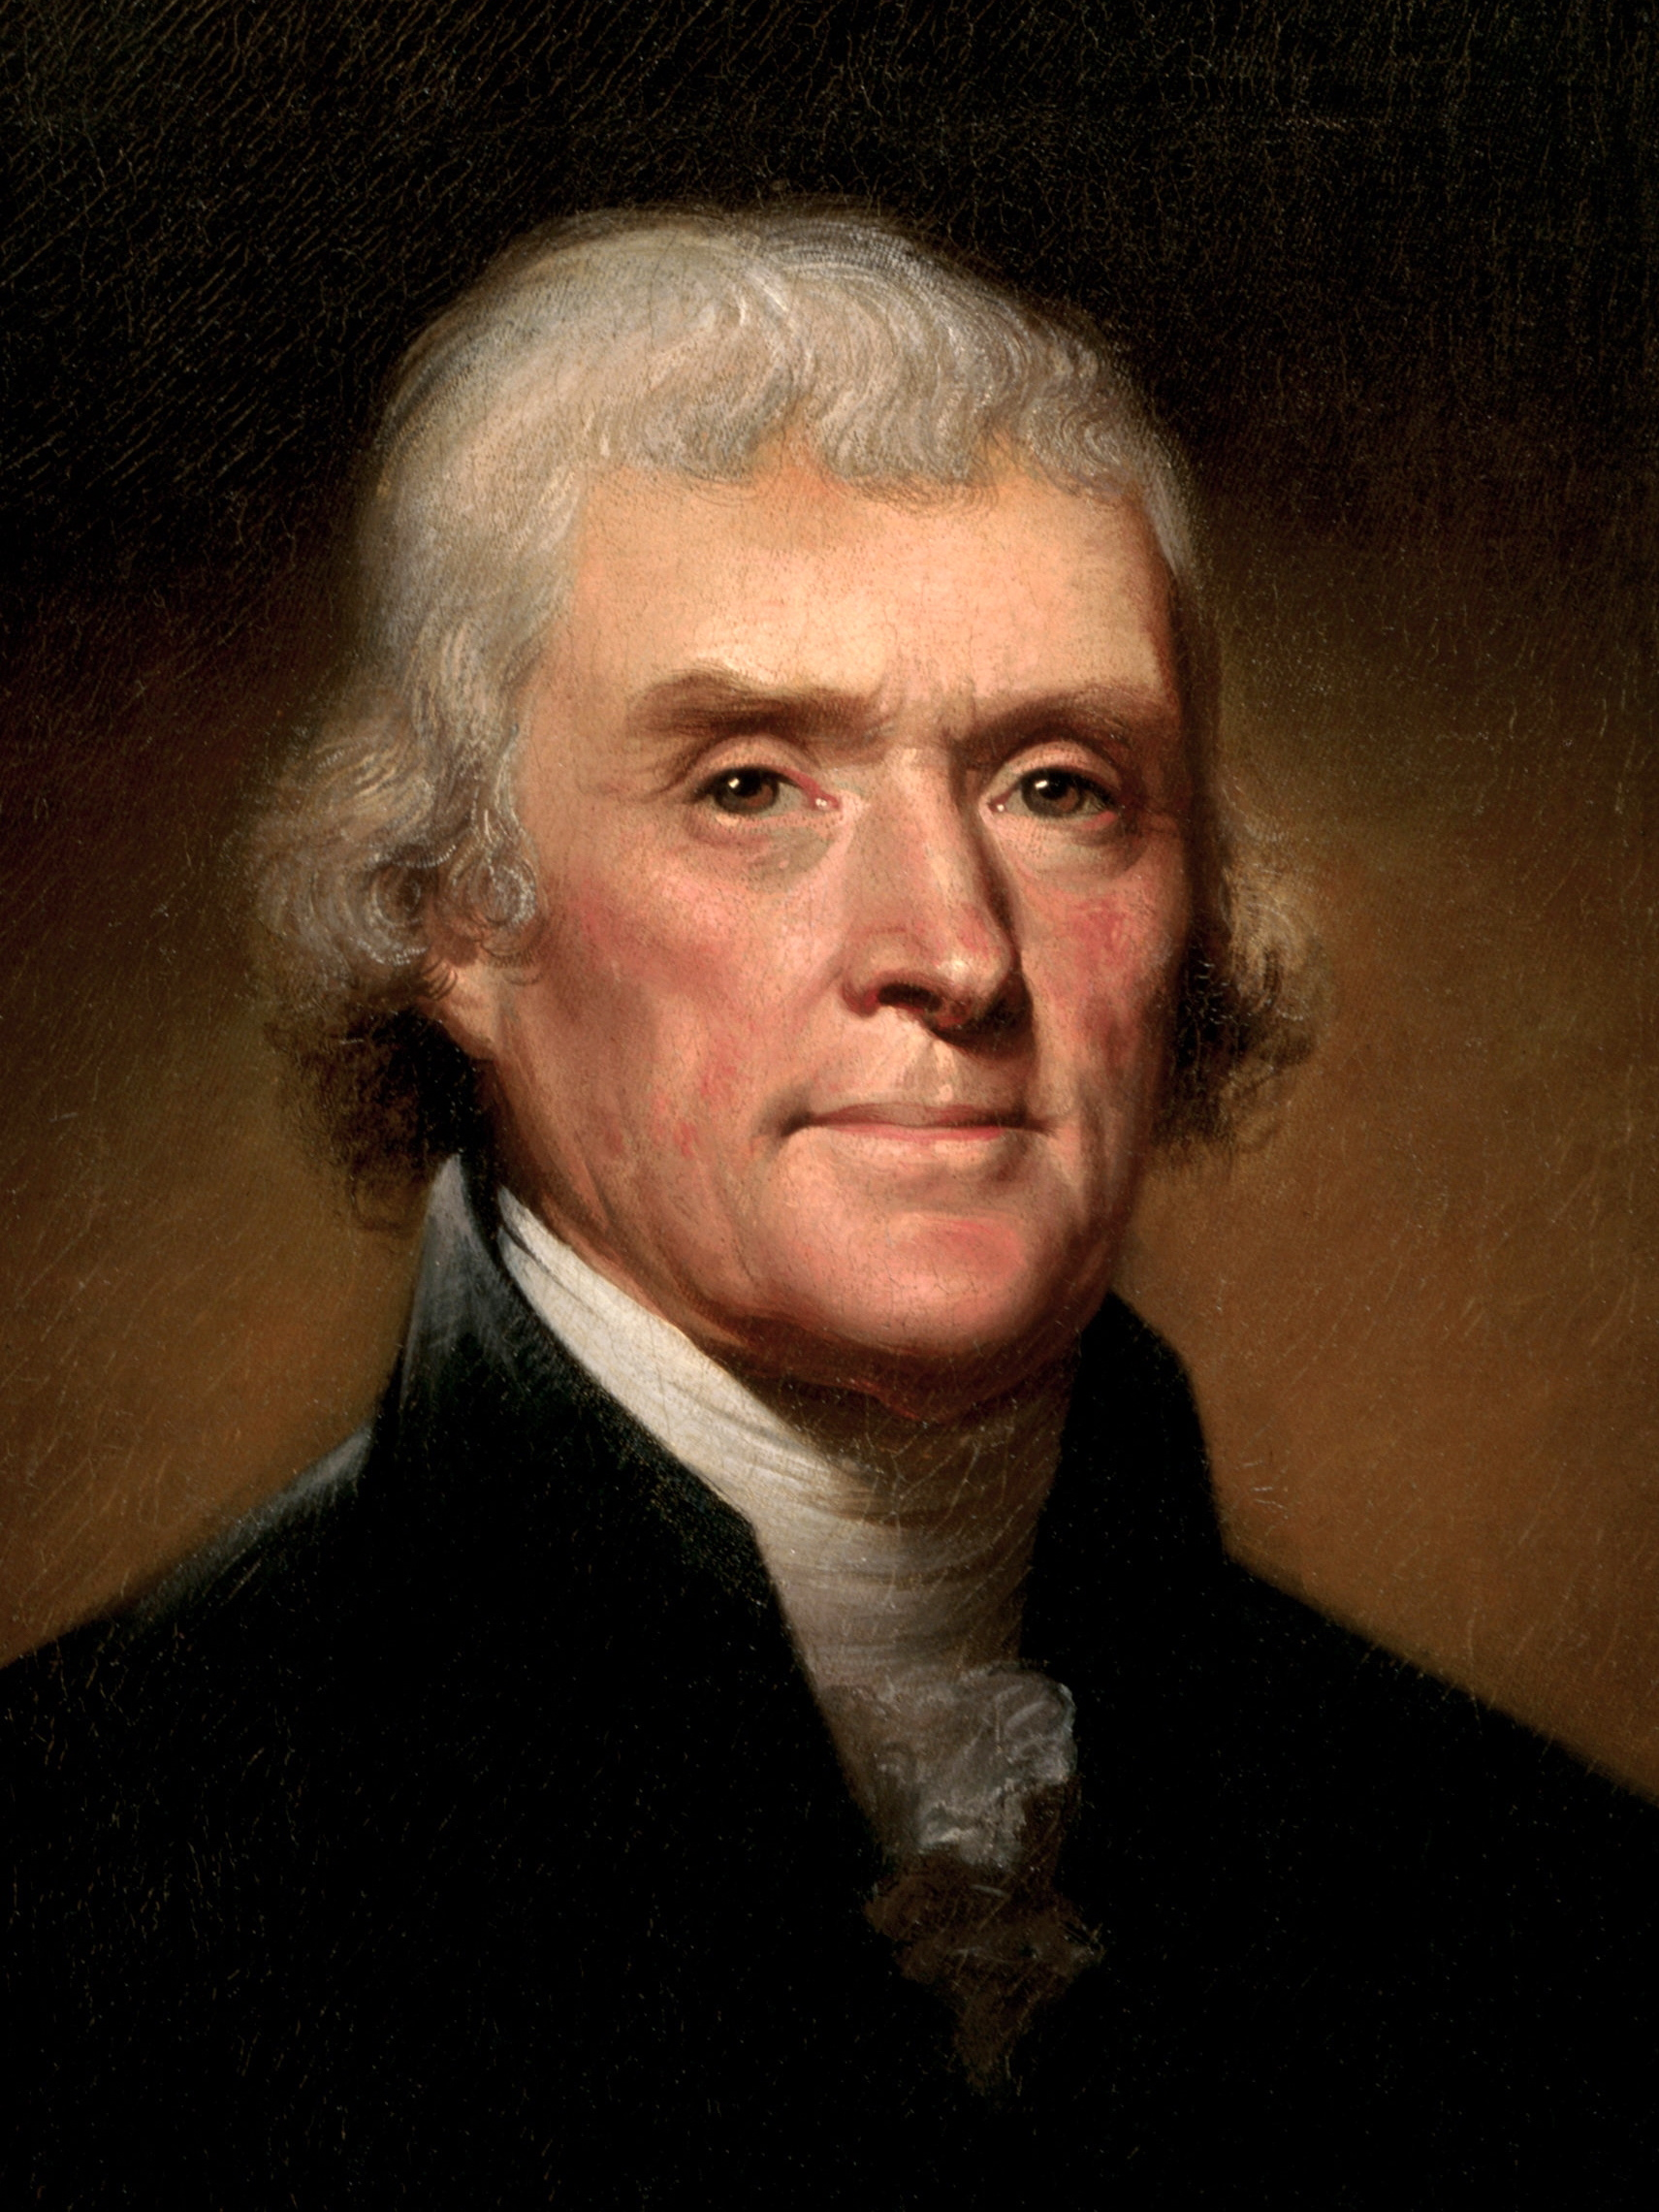
\includegraphics[height=0.75\textheight]{img/jefferson.png} \\
            Thomas Jefferson, 1824

        \column{0.5\textwidth}
            Men by their constitutions are naturally divided into two parties: \\
            \begin{enumerate}
                \item Those who fear and distrust the people, and wish to draw all powers from them into the hands of the higher classes.
                \item Those who identify themselves with the people, [and] have confidence in them.
            \end{enumerate}
    \end{columns}
\end{frame}

% REF: This window was commissioned in 1910 by George Bernard Shaw. It was stolen in 1978, recovered in 2005, and is now on display in the London School of Economics' Shaw library. http://www.lse.ac.uk/intranet/LSESocial/artsAndMusic/artOnCampus/Shaw%20Library.aspx
\begin{frame}{The World's Plan for Happiness}
    \centering
    \includegraphics[height=.7\textheight]{img/remold-it.jpg} \\
    Stained glass originally for the home of Sidney and Beatrice Webb, Baron and Baroness Passfield. Mrs. Webb coined the term ``collective bargaining'' in 1891.
% REF: "A Timeline of Events in Modern American Labor Relations", Federal Mediation and Conciliation Service, http://web.archive.org/web/20100802105125/http://www.fmcs.gov/internet/itemDetail.asp?categoryID=21&itemID=15810
\end{frame}

\begin{frame}{The World's Plan for Happiness}
    \centering
    \includegraphics[width=.9\textwidth]{img/remold-hammers.png} \\
\end{frame}

\begin{frame}{The World's Plan for Happiness}
    \centering
    \includegraphics[height=.9\textheight]{img/fabian-books.png} \\
\end{frame}

\begin{frame}{Government of Ancient Israel}
    \centering
    \includegraphics[width=0.75\textwidth]{img/moses.jpg} \\
    \only<1>{
        And Moses' father-in-law said unto him: Thou shalt teach them ordinances and laws, and shalt show them the way wherein they must walk and the work that they must do.
    }
    \only<2>{ Groups of tens, fifties, hundreds, thousands, to successfully govern three million people \\ }
%    \only<3>{ This became the basis of ``Common'', or ``People's'' Law \\ }
\end{frame}

\begin{frame}{Fundamental Principles of Socialism}
    \begin{enumerate}
        \item Government ownership or control of all land
        \item Government ownership or control of major industries
        \item Government control over labor
        \item Government ownership or control of communications and transportation
        \item Government control of all credit
        \item Government control of all insurance
        \item Government control of the educational system
        \item Elimination of the significance of the family
        \item Elimination of the significance of religion
        \item Establishment of a minimum wage
        \item A universal system of pensions
        \item Justified use of force where necessary to attain socialistic goals
        \item Graduated income tax
    \end{enumerate}
\end{frame}

\begin{frame}{Fundamental Principles of Freedom}
    \begin{enumerate}
        \item Thou shalt have no other gods before me
        \item Thou shalt not make unto thee any graven image
        \item Thou shalt not take the name of the Lord thy God in vain
        \item Remember the sabbath day, to keep it holy
        \item Honour thy father and thy mother
        \item Thou shalt not kill
        \item Thou shalt not commit adultery
        \item Thou shalt not steal
        \item Thou shalt not bear false witness against thy neighbour
        \item Thou shalt not covet
    \end{enumerate}
\end{frame}

% REF http://finance.townhall.com/columnists/maritanoon/2011/09/18/a_tree_party_rebellion/page/full
% REF http://www.alamogordonews.com/story/news/local/new-mexico/2015/10/08/otero-county-appealing-forest-lawsuit/73610574/
% REF http://www.justice.gov/usao-nm/pr/otero-county-resolution-authorizing-removal-trees-lincoln-national-forest-declared
\begin{frame}{Tree Party Rebellion}
    \begin{columns}[onlytextwidth]
        \column{0.5\textwidth}
            \centering
            \includegraphics[width=0.75\textwidth]{img/sheriff-benny-house1.jpg} \\
            Otero county, New Mexico \\

        \column{0.5\textwidth}
            \centering
            \only<1>{
            The US Forest Service prohibited most logging in New Mexico's
            national forests, to protect Mexican spotted owls. This led to
            dangerously intense forest fires.  In Sept, 2011, Sheriff House
            told the USFS that locals would begin to remove trees to reduce
            fire danger, and threatened to arrest any federal law enforcement
            that intervened.
            }
            \only<2>{
            In 2015, the US district court struck down the county resolution
            permitting the logging, saying it violated the Constitution's
            Supremacy clause.
            }
    \end{columns}
\end{frame}

\begin{frame}{Americans' Top 10 Fears}
    \centering
    \includegraphics[width=0.82\textwidth]{img/Top10Fears.jpg} \\
    Chapman University Survey of American Fears, Wave 2 (2015) \\
\end{frame}

% XXX get dates on stuff, like to show that Lincoln and Washington didn't choose fasces for their monuments' decorations

% "Who knows what this guy is carrying?"
\begin{frame}
    \centering
    \includegraphics[width=.9\textwidth]{img/fasces/fake-fasces.jpg} \\
    Catalonia (largely autonomous Spanish province), 2006 \\
\end{frame}

\begin{frame}
    \centering
    \includegraphics[height=.8\textheight]{img/fasces/flag-fasces.jpg} \\
\end{frame}

\begin{frame}
    \centering
    \includegraphics[width=.9\textwidth]{img/fasces/ows.jpg} \\
    Federal Hall, New York City \\
\end{frame}
\begin{frame}
    \centering
    \includegraphics[width=.9\textwidth]{img/fasces/fasces-stuff.jpg} \\
    Statue by John Quincy Adams Ward, 1882.
\end{frame}
\begin{frame}
    \centering
    \includegraphics[height=.8\textheight]{img/fasces/houdon-front.jpg} \\
    Statue by Jean-Antoine Houdon, completed 1791. Commissioned by Virgina's legislature, and on display at Colonial Williamsburg. \\
\end{frame}
\begin{frame}
    \centering
    \includegraphics[height=.8\textheight]{img/fasces/washington1.jpg} \\
    By Horatio Greenough, completed in 1840, and now found in the Smithsonian
    museum of American History. The base reads,``Horatio Greenough made this
    image as a great example of freedom, and will not survive without freedom
    itself.''
\end{frame}

\begin{frame}
    \begin{columns}[onlytextwidth]
        \column{0.5\textwidth}
            \centering
            \includegraphics[width=0.75\textwidth]{img/dime-usa-fasces-2.jpg} \\
            1916 - 1945 \\

        \column{0.5\textwidth}
            \centering
            \includegraphics[height=0.55\textheight]{img/fasces-copy.jpg} \\
            Roman Law\\

    \end{columns}
\end{frame}

\begin{frame}
    \centering
    \includegraphics[height=.8\textheight]{img/fasces/badge_description.jpg} \\
    Los Angeles Police Dept. badge, developed 1939 - 1941 \\
\end{frame}
\begin{frame}
    \centering
    \includegraphics[height=.8\textheight]{img/fasces/coin.jpg} \\
    Italian East Africa Campaign medal, 1936 \\
\end{frame}
\begin{frame}
    \centering
    \includegraphics[height=.8\textheight]{img/fasces/fasces13.jpg} \\
    Adopted 1877. Text reads ``Union and Consitution''. Colorado's state website claims ``The Roman fasces is the insignia of a republican form of government\ldots The axe symbolizes authority and leadership.'' \\
\end{frame}
\begin{frame}
    \centering
    \includegraphics[height=.8\textheight]{img/fasces/fasces5coin.jpg} \\
\end{frame}

\begin{frame}
    \centering
    \includegraphics[height=.8\textheight]{img/fasces/french-republic-symbol.png} \\
    National Symbol of France, adopted 1953. This symbol is used to represent France in the U.N. Assembly building. \\
\end{frame}
\begin{frame}
    \centering
    \includegraphics[height=.8\textheight]{img/fasces/italy-fasces-coin.jpg} \\
    Italian 5 lira piece, 1928 \\
\end{frame}

\begin{frame}
    \centering
    \includegraphics[width=.9\textwidth]{img/obama-fasces.jpg} \\
\end{frame}

\begin{frame}
    \centering
    \includegraphics[width=.9\textwidth]{img/fasces/fasces_congress.jpg} \\
\end{frame}

\begin{frame}
    \centering
    \includegraphics[height=.9\textheight]{img/fasces/jfk.jpg} \\
\end{frame}

\begin{frame}{1914}
    \centering
    \includegraphics[width=.9\textwidth]{img/lincoln-memorial.jpg} \\
\end{frame}

\begin{frame}
    \begin{columns}[onlytextwidth]
        \column{0.5\textwidth}
            \centering
            \includegraphics[width=0.75\textwidth]{img/americas-caesar.png} \\

        \column{0.5\textwidth}
            \begin{block}{America's Caesar}
                The Decline and Fall of Republican Government in the United States of America
            \end{block}
    \end{columns}
\end{frame}

\begin{frame}
    \centering
    \includegraphics[width=.9\textwidth]{img/fasces/lincoln_fasces.jpg} \\
\end{frame}
\begin{frame}
    \centering
    \includegraphics[width=.9\textwidth]{img/fasces/manhole.JPG} \\
\end{frame}

% REF http://720mpreunion.org/history/assets/Corps%20History/mp_history.html
\begin{frame}
    \begin{columns}[onlytextwidth]
        \column{0.48\textwidth}
            \includegraphics[width=0.8\textwidth]{img/18th-mp-brigade-badge.jpg} \\
            Combat Service Identification badge, 18th Military Police Brigade \\

        \column{0.04\textwidth}
            \\

        \column{0.48\textwidth}
            \includegraphics[width=0.8\textwidth]{img/army-mp-crest.jpg} \\
            Army Military Police Corps crest \\
    \end{columns}
\end{frame}

% REF 26 U.S. Code § 7441, http://www.legisworks.org/GPO/STATUTE-83-Pg487.pdf
\begin{frame}
    \centering
    \includegraphics[height=.8\textheight]{img/fasces/tax-court.png} \\
    The Tax Court took its present form in 1969 \\
\end{frame}

\begin{frame}
    \centering
    \includegraphics[height=.8\textheight]{img/fasces/teut1.jpg} \\
    Detail of frieze in the U.S. Capitol rotunda. The frieze was designed in 1859 and begun in 1877, but wasn't fully complete until 1953. \\
\end{frame}
\begin{frame}
    \centering
    \includegraphics[width=.9\textwidth]{img/fasces/tunnel.jpg} \\
\end{frame}
\begin{frame}
    \centering
    \includegraphics[width=.9\textwidth]{img/reich-stamp.png} \\
\end{frame}

\begin{frame}
    \centering
    \includegraphics[width=.9\textwidth]{img/supremecourtfasces.jpg} \\
    \large{ Front of the Supreme Court building } \\
\end{frame}

\begin{frame}
    \centering
    \includegraphics[height=.85\textheight]{img/fasces_west_supcourt.jpg} \\
    \large{ On November 28, 2008, 172 pounds of this facade fell four stories to land on the steps of the court } \\
\end{frame}

% XXX Get dates on the fasces pictures, and some idea of who designed these monuments (e.g. lincoln, sup. court bldg.)
% XXX The story of the great seal is interesting. Jefferson had an idea for it already.
\begin{frame}
    \centering
    \includegraphics[width=.98\textwidth]{img/supcourt-east-clipped.png} \\
    \large{ Rear of the Supreme Court building } \\
\end{frame}
\begin{frame}
    \centering
    \includegraphics[height=.9\textheight]{img/moses_east_supcourt.jpg} \\
    \large{ Rear of the Supreme Court building } \\
\end{frame}

% REF Glassroth v. Moore, CV-01-T-1268-N, 229 F. Supp. 2d 1290
\begin{frame}
            \centering
            \includegraphics[width=.65\textwidth]{img/10-commandments.jpg} \\
            \only<1>{
            Alabama Supreme Court Chief Justice Roy Moore commissioned this 2.5 ton
            monument of the Ten Commandments, and it was installed in 2001.}
            \only<2>{Within
            three months, the ACLU, Southern Poverty Law Center, and others filed
            suit in federal court to have the monument removed, claiming it
            ``sends a message'' that the state government ``endorses the practice
            of religion''.}
            \only<3>{The suit succeeded,
            and the monument was removed in 2003.}
\end{frame}

\begin{frame}{Two Contending Forces}
    \begin{columns}[onlytextwidth]
        \column{0.5\textwidth}
            \begin{varblock}[0.9\textwidth]{}\huge{ \centering Sovereignty of the National Government \\}\end{varblock}

        \column{0.5\textwidth}
            \begin{varblock}[0.9\textwidth]{}\huge{ \centering Sovereignty of the individual States \\}\end{varblock}
    \end{columns}
    \textbf{\huge{ \color{red}
        \Put(155,120){v.}
    }}
\end{frame}
    
\begin{frame}{Two Contending Forces}
    \begin{columns}[onlytextwidth]
        \column{0.5\textwidth}
            \includegraphics[width=0.8\textwidth]{img/federalistpapers.jpg} \\

        \column{0.5\textwidth}
            \includegraphics[width=0.8\textwidth]{img/anti-federalist.jpg} \\
    \end{columns}
\end{frame}

% XXX 1828 dictionary, def. of decimate
\begin{frame}{Theban Legion}
    \centering
    \includegraphics[height=0.7\textheight]{img/theban-1.jpg} \\
    Abbaye de Saint-Maurice, Switzerland. Stained glass by Swiss artist Edmond Bille. \\
\end{frame}

% XXX Better mencken picture? Kinda pixellated
\myquote{H.L. Mencken, Baltimore Sun, 12 Feb 1923}{img/mencken.jpg}{``The fact is that the average man's love of liberty is nine-tenths imaginary, exactly like his love of sense, justice and truth.''}
\myquote{H.L. Mencken, Baltimore Sun, 12 Feb 1923}{img/lonely.jpg}{``\ldots He is not actually happy when free; he is uncomfortable, a bit alarmed, and intolerably lonely.''}
\myquote{H.L. Mencken, Baltimore Sun, 12 Feb 1923}{img/black-sheep.jpg}{``\ldots Liberty is not a thing for the great masses of men. It is the exclusive possession of a small and disreputable minority, like knowledge, courage and honor.''}
% XXX Is there some other hanging engraving that is a better story
\myquote{H.L. Mencken, Baltimore Sun, 12 Feb 1923}{img/Jacob-henry-harmon-hanging-1862.jpg}{``\ldots It takes a special sort of man to understand and enjoy liberty — and he is usually an outlaw in democratic societies.''}

% XXX what's the story here? What were the Danbury's actually complaining about? Also, this quote is too long, and loses people. cf. Jeremy. And add pictures.
\begin{frame}{Danbury Baptist Association, to Thomas Jefferson, 7 Oct 1801}
    ``\ldots what religious privileges we enjoy (as a minor part of the State) we enjoy as favors granted, and not as inalienable rights to: and these favors we received at the expense of such degrading acknowledgements, as are inconsistent with the rights of freemen.''
\end{frame}

% XXX Include somewhere "Do all that you've said you're going to do, and do not infringe on other people or their property" Find Richard Mayberry. Or perhaps the "don't hit other people or take their stuff"
% Include "Uncle Eric" series. We need a handout with references, and that can go on there.

% XXX Notes on Jefferson bible, to counter "deists don't want Christ" stuff. Stuff from Franklin, as well, who liked scripture even if he was atheistish
\myquote{Thomas Jefferson, to Danbury Baptist Association, 7 Oct 1801}{img/jefferson.png}{``Believing with you that religion is a matter which lies solely between Man and his God, that he owes account to none other for his faith or his worship, \ldots''}
\myquote{Thomas Jefferson, to Danbury Baptist Association, 7 Oct 1801}{img/coexist.png}{``\ldots that the legitimate powers of government reach actions only, and not opinions, \ldots''}
\myquote{Thomas Jefferson, to Danbury Baptist Association, 7 Oct 1801}{img/great-wall.jpg}{``\ldots I contemplate with sovereign reverence that act of the whole American people which declared that their legislature should 'make no law respecting an establishment of religion, or prohibiting the free exercise thereof,' thus building \textbf{a wall of separation between Church and State} \ldots''}
\myquote{Thomas Jefferson, to Danbury Baptist Association, 7 Oct 1801}{img/jefferson.png}{``\ldots Adhering to this
expression of the supreme will of the nation in behalf of the rights of
conscience, I shall see with sincere satisfaction the progress of those
sentiments which tend to restore to man all his natural rights, convinced
\textbf{he has no natural right in opposition to his social duties}.''}
% XXX Nail what Jefferson means by social duties. It's not "social justice". Does Jefferson tell us we have a social duty to make sure everyone's treated fairly, for instance?

% XXX MOAR KWOTES, and references
\begin{frame}{Reynolds v. US, 1878}
    The Supreme Court decided that whatever Jefferson said is ``almost as an authoritative declaration'' of what the Constitution means, because Jefferson wrote it.
\end{frame}

\begin{frame}{Reynolds v. US, 1878}
    \centering
    \includegraphics[width=0.75\textwidth]{img/Joseph-F-Smith-family.png} \\
    Then the Supreme Court decided objection to polygamy was a social duty, so forbidding it was Constitutional.
\end{frame}

% XXX More examples of people taking "wall of separation" too far, and out of context. My contention is that Reynolds didn't quite do that, but others have.
\begin{frame}{Wall of Separation}
    \centering
    \includegraphics[width=0.75\textwidth]{img/great-wall.jpg} \\
    Now everyone talks about a ``wall of separation'' without any of the context.
\end{frame}

\begin{frame}
    \centering
    \includegraphics[height=0.95\textheight]{img/christ-statue.jpg} \\
\end{frame}

% XXX Another picture of statue, with background

% XXX More scriptures; Steve used some of these.
\myquote{Isaiah 5:13; Image of ``Christ the King'' statue, in Świebodzin, Poland}{img/christ-statue.jpg}{``Therefore my people are gone into captivity, because they have no knowledge: and their honourable men are famished, and their multitude dried up with thirst.''}

\end{document}

% Steve video starts at 32:43 ("two things I want to share") until 36:58
